\RequirePackage[l2tabu, orthodox]{nag}	% To be warned of outdated commands
\documentclass[paper=a4, 12pt]{scrartcl}
\usepackage{fontspec}
\usepackage{setspace}			% For line spacing
\usepackage[usenames,dvipsnames]{color}	% For colorful text
\usepackage[margin=10pt,font=small,labelfont=bf,labelsep=endash,format=plain]{caption}
\usepackage{microtype}			% For nicer spacing
\usepackage{graphicx}
\usepackage{bigfoot}
%\usepackage{siunitx}			% For units

\usepackage[colorlinks=true,
				linkcolor=black,
				citecolor=black,
				filecolor=black,
				urlcolor=black,
				pdfusetitle]{hyperref}	% Links and URLs
\urlstyle{rm}					% URLs are written in roman instead of typewriter

\frenchspacing					% No extended space after sentences
\clubpenalty = 10000
\widowpenalty = 10000
\displaywidowpenalty = 10000

\setromanfont{Linux Libertine O}
\setsansfont{Linux Biolinum O}
\setmonofont{FreeMono}

\newcommand{\xxx}[1]{\textbf{\textcolor{red}{#1}}}	% Emphasizing parts to do

%\definecolor{lightgrey}{rgb}{0.8,0.8,0.8}

%\newcommand{\cmd}[1]{\texttt{\colorbox{lightgrey}{> #1}}}




% % % % % % % % % % % % % % Heeere we go! % % % % % % % % % % % % % % %

\begin{document}

\title{Report}
\subtitle{INF-9380}
\author{Mathias Bockwoldt}
\date{20.05.2016}

\maketitle

\onehalfspacing

The repository with all files, including this report, can be found here: \url{https://github.com/mathiasbockwoldt/inf9380exam.git} .

\section{ChIP-Seq SLURM workflow}

All files for this part are in the folder \texttt{chipseq-part}.

\subsection{Bowtie and MPI (part 1)}

All files for this part are in the folder \texttt{ex1\_bowtie}.

I ran Bowtie five times in serial mode to get a baseline for the execution time. Afterwards I ran Bowtie using MPI as shown in the example script with one to 16 cores five times each. Everything was run on a single node with all 16 cores allocated to my script. Hence, there should not have been any delay by inter-node data transmission. The script for running Bowtie with and without MPI is given in \texttt{run.slurm} (calling the MPI script in a loop) and \texttt{mpirun\_script.sh} (calling Bowtie with MPI). The runtimes were measured by the \texttt{time} command and saved in \texttt{times.ods}. As the average times varied quite heavily, I chose the minimum time of five calls for an estimate of the runtime. The speedup is shown in fig \ref{fig:chipseq-bowtie} using \texttt{real} times.

\begin{figure}[ht]
	\centering
		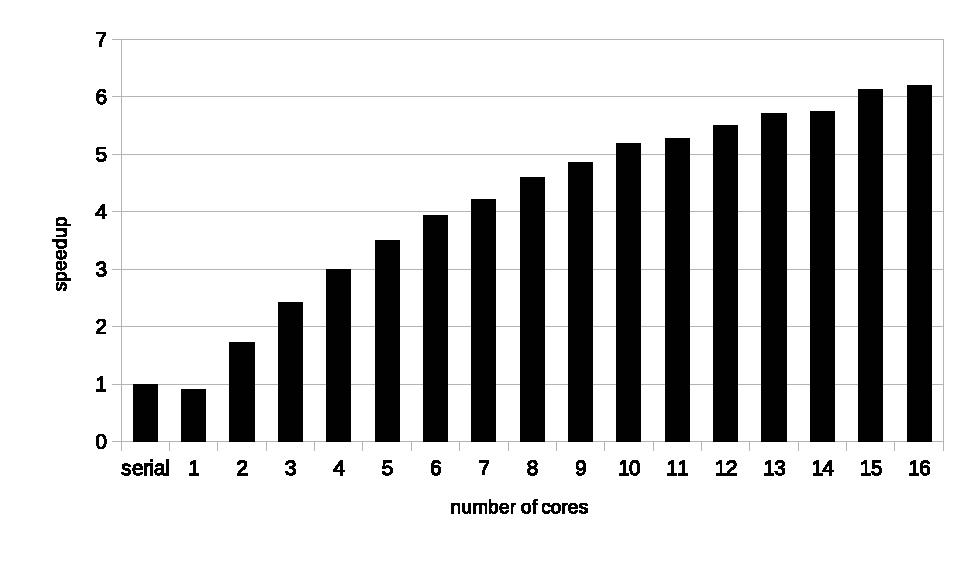
\includegraphics[width=0.8\textwidth]{chipseq-bowtie}
	\caption{The speedup of Bowtie with MPI. Serial is Bowtie without MPI whose speedup is set to 1. The MPI with only one processor has a speedup lower than 1 due to the overhead of parallelization.}
	\label{fig:chipseq-bowtie}
\end{figure}

The speedup is as expected. The execution gets faster with each additional core, but the increase in speed declines with the number of cores due to the parallelizing overhead. When using more cores, the file must be split into more chunks, more processes must be spawned and more result files must be concatenated after execution. With few processes, this pays off, but the more processes are spawned, the less pronounced is the speedup.

A \texttt{diff} result of the output file of the serial Bowtie and Bowtie using MPI with 16 cores shows that the file contents themselves are identical. Only the header lines repeat (one header for each process). This is easily solvable for example using \texttt{awk} to remove the excessive headers\footnote{\verb&awk 'NR <= 3 || !/^@/'&}.

\subsection{SLURM scripts (parts 2 to 4)}

All serial files are in the folder \texttt{ex2\_serial} and the parallelized files (using \texttt{arrayrun}) in \texttt{ex3\_parallel}.

SLURM scripts were written to follow the workflow given in the course. This resulted in eleven scripts plus one for preparation of the data and one R script. I did not use the SCRATCH folder in any of the scripts as the files were very small. If the files were bigger I would of course take the effort to copy all relevant files for a given script to SCRATCH and copy all relevant output files back to the original directory.

Firstly, all scripts were run ones with generous memory and time demands to find out the actual memory consumption and runtime that were used to adjust the \texttt{sbatch} directives accordingly. Runtimes were given by the SLURM log files. I wrote an SDAG file to start the workflow given in fig \ref{fig:chipseq-workflow}. The whole workflow was started three times with Bowtie using MPI (including the little \texttt{awk} script to remove excessive headers) and three times using serial Bowtie. The times used for each script and the total times measured by getting the start time of the first script and the end time of the last script (usually \texttt{makeBigWig}). The results were saved in \texttt{runtimes.ods} and shown in fig \ref{fig:chipseq-runtimes}.

\begin{figure}[ht]
	\centering
		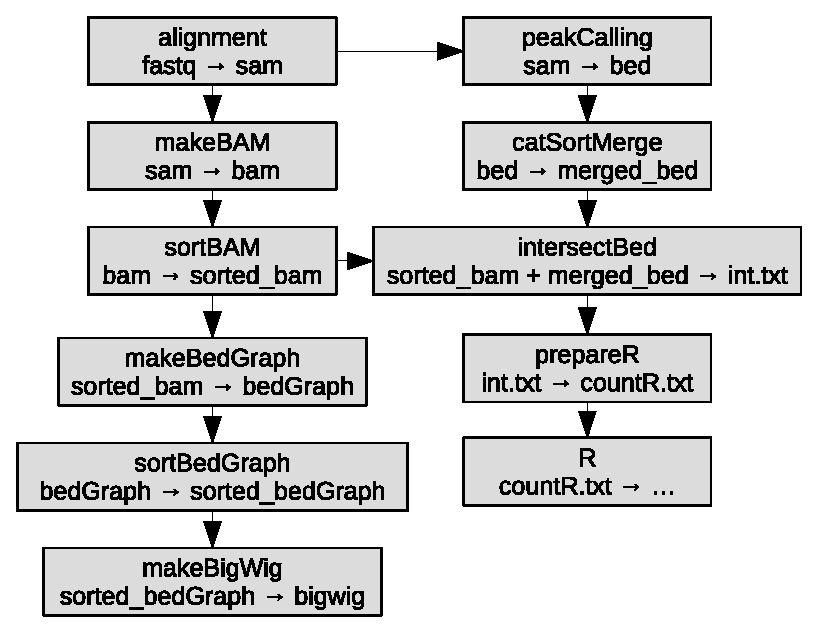
\includegraphics[width=0.6\textwidth]{chipseq-workflow}
	\caption{The workflow used for the chipseq part. The first line shows the name of the SLURM script, the second line shows the file types that are used and produced.}
	\label{fig:chipseq-workflow}
\end{figure}

\begin{figure}[ht]
	\centering
		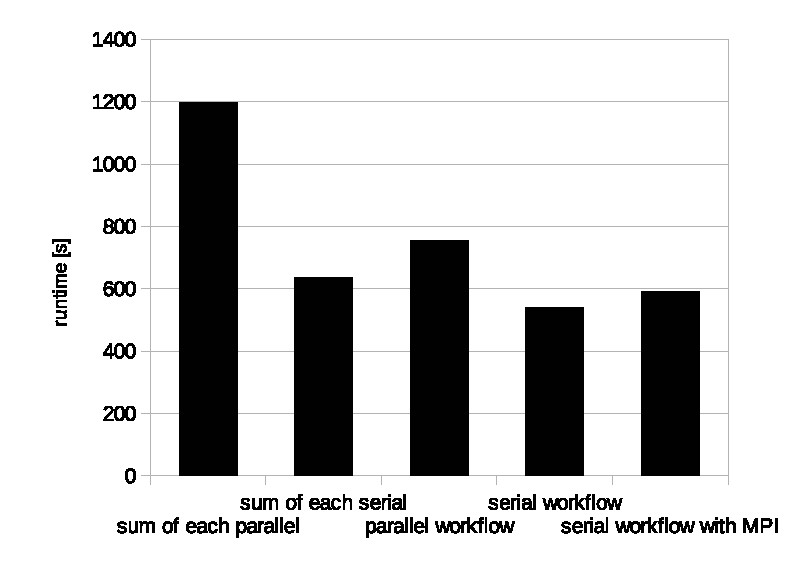
\includegraphics[width=0.7\textwidth]{chipseq-runtimes}
	\caption{Runtimes for different variations of the chipseq workflow. The first two bars show the sum of runtimes of each script using \texttt{arrayrun} (first bar) or not using any parallelization (second bar). The other three bars show the actual runtimes of whole workflows from the start of the first script until the end of the last script. Each value depicted here is the minimum of three executions of the respective workflows.}
	\label{fig:chipseq-runtimes}
\end{figure}

Most scripts were rewritten to work with \texttt{arrayrun}. Each script that should be run in parallel was divided in a submit script (\texttt{sub\_*.slurm}) and a worker script (\texttt{work\_*.slurm}). The SDAG script was adapted accordingly. The new parallelized workflow was run three times and the results saved in \texttt{runtimes.ods} and shown in fig \ref{fig:chipseq-runtimes}.

Interestingly, all arrayrun scripts took between 120 and 150 seconds (2 to 2.5 minutes), although the serial counterparts, except for the Bowtie and the bedGraph sorting step took considerably less time. As all arrayrun scripts took a very similar (and relatively long) time, I assume that arrayrun has either a huge overhead or only polls for results every few minutes. As such, arrayrun is not suitable for tasks that take less than about three minutes when run in serial. In the two cases where the serial SLURM scripts took more than 150 seconds, arrayrun resulted in a speedup but only to a very limited extend.

Both workflows without MPI (i.e. serial and parallel) coordinated with SDAG were faster than the sum of their parts (columns one vs. three and two vs. four, respectively, in fig \ref{fig:chipseq-runtimes}), although the runtime for the whole workflow included the time waiting for allocation of resources. The speedup is much larger for the parallel workflow than for the serial one. This is due to the longer runtimes of the parallel scripts compared to the serial scripts, such that the overhead of running the workflow (especially the time for resource allocation) is relatively less for the parallel than for the serial workflows.

Running Bowtie with MPI in eight processes resulted in slightly longer total workflow runtimes than without any parallelization. This is probably again due to the larger overhead of MPI parallelization (splitting, distribution, and merging of files) compared to the small file sizes used in this exam.

In general, larger files would have supported the use of parallelization more than the relatively small files used in the course.

\subsection{Setup manual (part 5)}

This manual assumes that all relevant files are in the same directories\footnote{\texttt{/work/}\allowbreak\texttt{projects/}\texttt{norbis/}\allowbreak\texttt{workflows/}\allowbreak\texttt{chip/}} as they were during the course. Furthermore, it assumes execution on Stallo as well as all used programs being installed properly or in the course directory.

\begin{flushleft}
\begin{enumerate}
\item clone my git repository to Abel (\texttt{git} \texttt{clone} \texttt{https://}\allowbreak\texttt{github.com/}\allowbreak\texttt{mathiasbockwoldt/}\allowbreak\texttt{inf9380exam.git})
\item navigate to the directory \texttt{chipseq-part/}\allowbreak\texttt{ex2\_serial} or \texttt{chipseq-part/}\allowbreak\texttt{ex3\_parallel} for the serial and parallel part, respectively
\item prepare directory structure and index reference genome by running \texttt{sbatch} \texttt{preparation.slurm}
\item load the sdag module (\texttt{module} \texttt{load} \texttt{sdag})
\item run the desired workflow (\texttt{chipseq.sdag} for both, parallel and serial, or \texttt{chipseq\_withMPI.sdag} in the serial folder for execution without arrayrun but with MPI for the Bowtie part \texttt{sdag} \texttt{chipseq.sdag})
\end{enumerate}
\end{flushleft}


\section{Differences between two VCF files}

All files for this part are in the folder \texttt{python-part}.

The Python 3 code I wrote to find differences between two VCF files is very crude and unflexible but it gets its job done.

First the control and subject files are read into Python lists. Afterwards, these are turned into dictionaries (key-value pairs). Each key is a tuple of the chromosome, the position on the chromosome and the alternative base. The value is the whole line of the respective SNP. For each dictionary, a Python set is generated of the dictionary keys. These two sets are then subtracted from each other to result in a new set with only the keys that are in the subject but not in the control. Based on this new set, a dictionary is returned with only the values whose keys are in the new set. All lines in that resulted dictionary are finally written to disk.

The parallel script does in principle the same, but splits the input files by chromosome and initializes a Python multiprocessing worker pool to send the data for each chromosome to a separate process. After processing the data, the results are written serially to a single file.

The fastest run of the serial program took 150~ms \texttt{real} and 124~ms \texttt{user} time, whereas the fastest run of the parallel version needed 233~ms and 184~ms \texttt{real} and \texttt{user} time, respectively. The average times were close to these values. Thus, the parallel execution took more time than the serial execution. This is due to the overhead of splitting and merging the working packages as well as the initialization of the worker pool. The parallel script would probably be faster than the serial script when used with larger files than the given test files.

\section{Galaxy and Docker}

All files for this part are in the folder \texttt{galaxy-part}.

I decided to write a wrapper for the software \texttt{Haystack}\footnote{\url{http://haystack.mocklerlab.org}}. In my PhD project, I use none of the programs in the list given for this exam and I thought it would be better to use something, I actually work with. Haystack is a Perl script to identify oscillating genes in gene expression data. The program call is not as complicated as the example programs, but with seven parameters it fulfills the demand for more than five parameters and still kept me busy for quite some hours.

I got a basic xml file by using \texttt{planemo} \texttt{tool\_init} with many parameters. This xml file was then filled with additional data and two tests. After some corrections, the Planemo linting tool revealed no obvious failures in the file. Also the tests with \texttt{planemo} \texttt{test} passed.

After creating a \texttt{.shed.yaml} file and filling it with necessary infos, I created the repository \texttt{haystack} in the Test Tool Shed\footnote{\url{https://testtoolshed.g2.bx.psu.edu}} where I could then upload the tool with \texttt{planemo} \texttt{shed\_upload}.

I wrote the necessary files for extending the Docker Galaxy flavour and built it with \texttt{docker} \texttt{build}, ran it and pushed it to DockerHub where it can be found under \texttt{mathiboc/}\allowbreak\texttt{galaxyhaystack}. I had a problem with a Perl dependency. Haystack needs the Perl module Statistics::Distributions which was installed on my Computer, so I did not get any failures while testing the Galaxy tool on my computer. However, the module is not installed on the basic Galaxy Docker image. I tried to define the dependecies such that the module is installed automatically (using a \texttt{tool\_dependencies.xml} file that can still be found in the git repository), but when starting the Haystack-flavoured Galaxy in Docker, I always got the error message that the required module is not available. After a lot of unsuccessful reading and trying, I decided to resolve the dependecies by hand in the \texttt{Dockerfile} (lines 17 and 18). I'm aware of that this is not the best practice but the deadline forced me to compromise at some point.

\end{document}
